\begin{figure}[t]
\centering
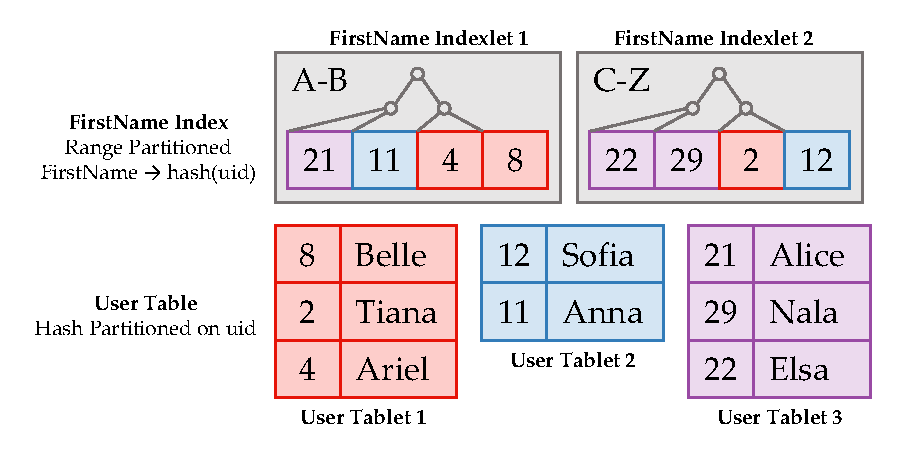
\includegraphics[width=1.0\columnwidth]{figures/ramcloud-index.pdf}
\caption{Index partitioning. Records are stored in unordered tables that can be
  split into tablets on different servers, partitioned on the primary key hash.
  Indexes can be range partitioned into indexlets; indexes only contain primary
  key hashes. Range scans require first fetching a list of hashes from an
  indexlet, then multigets for those hashes to the tablet servers to fetch the
  actual records.  A lookup or scan operation is (usually) handled by one
  server, but tables and their indexes can be split and scaled independently.}
\label{fig:index}
\end{figure}
